Laser Harp consists of four layers. The first layer is the power system, which is going to act as a power source for the device and consists of battery or similar power source. Second layer is frames and components which consists of laser beams, receptors, mister and speaker.  Receptors are going to identify the interference in the laser beam and send the signal towards MIDI converter.  Mister is being used for visibility whereas speakers are for audio output.  Then, we have MIDI converter which is going to receive signals from the receptors and encode those signals as MIDI signals.  Finally, the last layer is the sound module which is going to decode the MIDI signals, pass the resulting outcome to fluid synth which in turn sends the audio signals to speakers via sound card.\\

The laser harp instrument's UI consists of a touch screen monitor which allows the users to change the sound fonts as well as change the reverberations, gain,etc. of the outgoing sound.

\begin{figure}[h!]
	\centering
 	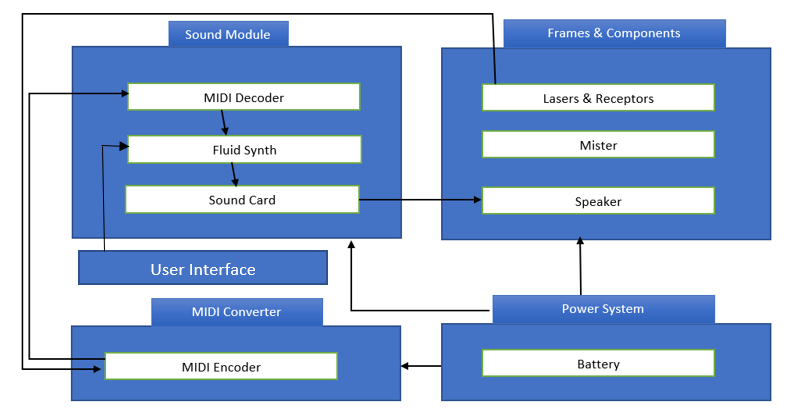
\includegraphics[width=0.90\textwidth]{images/data_flow.png}
 \caption{System architecture}
\end{figure}
